\section{Optimierung der Parameter des BDT-Algorithmus}
Um einen höheren AMS-Wert zu erreichen, variierten wir folgende Parameter des BDT-Algorithmus.
\begin{equation}
\begin{split}
 \mbox{\textit{PDFInterpolMVAPdf}} &\in \{ \mbox{ Spline1,  Spline2, Spline3}  \}  \\
 \mbox{\textit{NsmoothMVAPdf}} &\in \{ \mbox{5,10,15, \ldots, 195} \}
\end{split}
\end{equation}

\begin{figure}[htp]
\begin{center}
  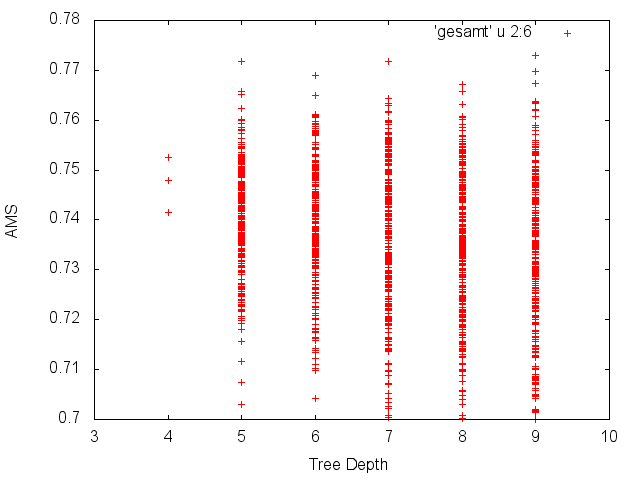
\includegraphics[width=0.7\linewidth]{sections/parameter_optimization_bdt/Depth.png}
 \caption[]{}
\label{fig:bdt_Depth}
\end{center}
\end{figure}

\begin{figure}[htp]
\begin{center}
  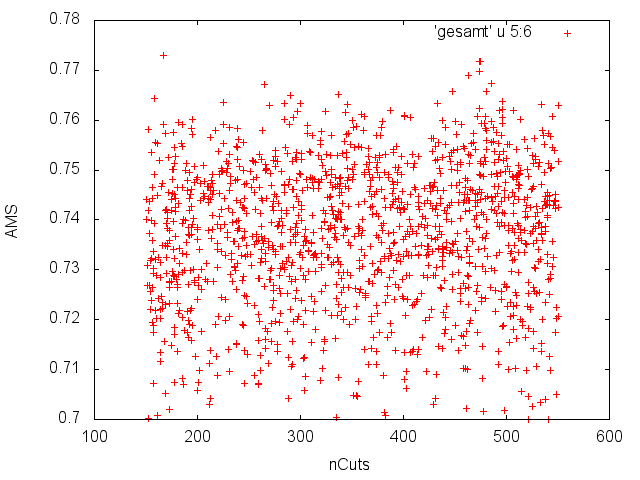
\includegraphics[width=0.7\linewidth]{sections/parameter_optimization_bdt/nCuts.png}
 \caption[]{}
\label{fig:bdt_nCuts}
\end{center}
\end{figure}


\begin{figure}[htp]
\begin{center}
  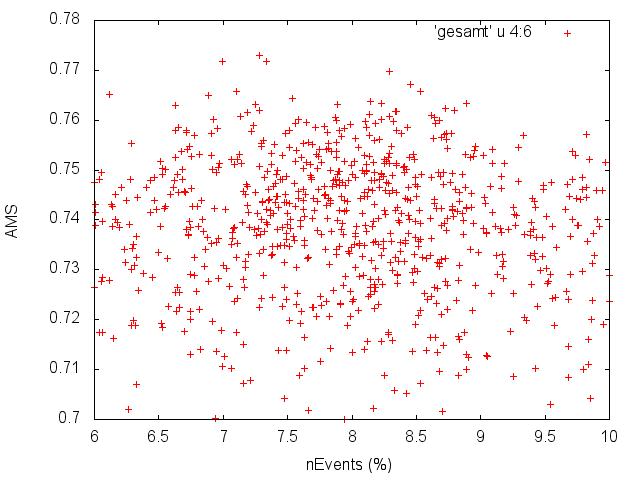
\includegraphics[width=0.7\linewidth]{sections/parameter_optimization_bdt/nEvents.png}
 \caption[]{}
\label{fig:bdt_nEvents}
\end{center}
\end{figure}

\begin{figure}[htp]
\begin{center}
  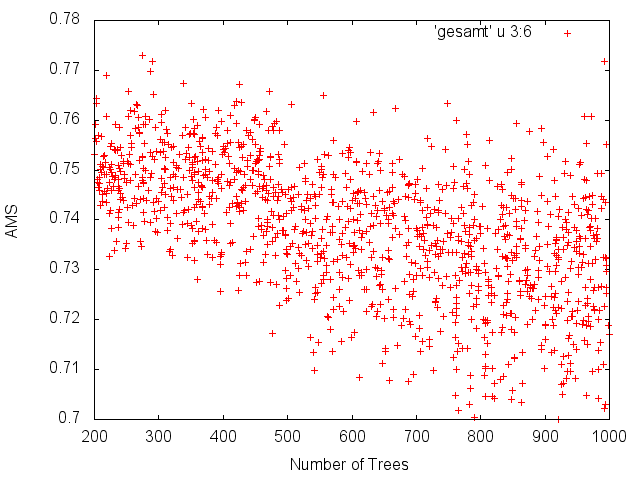
\includegraphics[width=0.7\linewidth]{sections/parameter_optimization_bdt/Nt.png}
 \caption[]{}
\label{fig:bdt_Nt}
\end{center}
\end{figure}

\begin{figure}[htp]
\begin{center}
  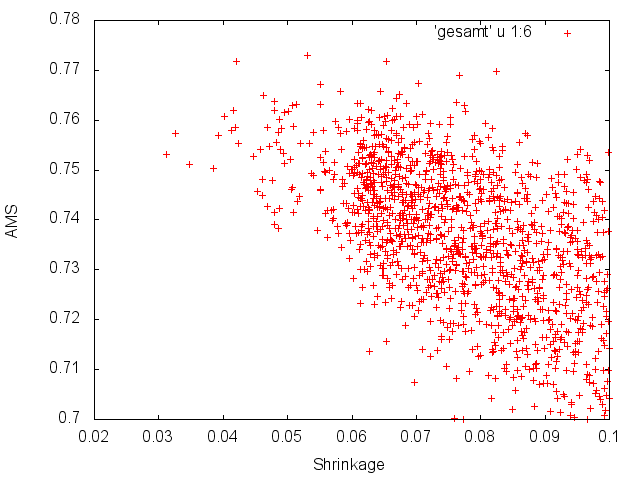
\includegraphics[width=0.7\linewidth]{sections/parameter_optimization_bdt/Shrinkage.png}
 \caption[]{}
\label{fig:bdt_Shrinkage}
\end{center}
\end{figure}